%cs-uwb_intro.tex

\begin{figure}[!t]
\centering
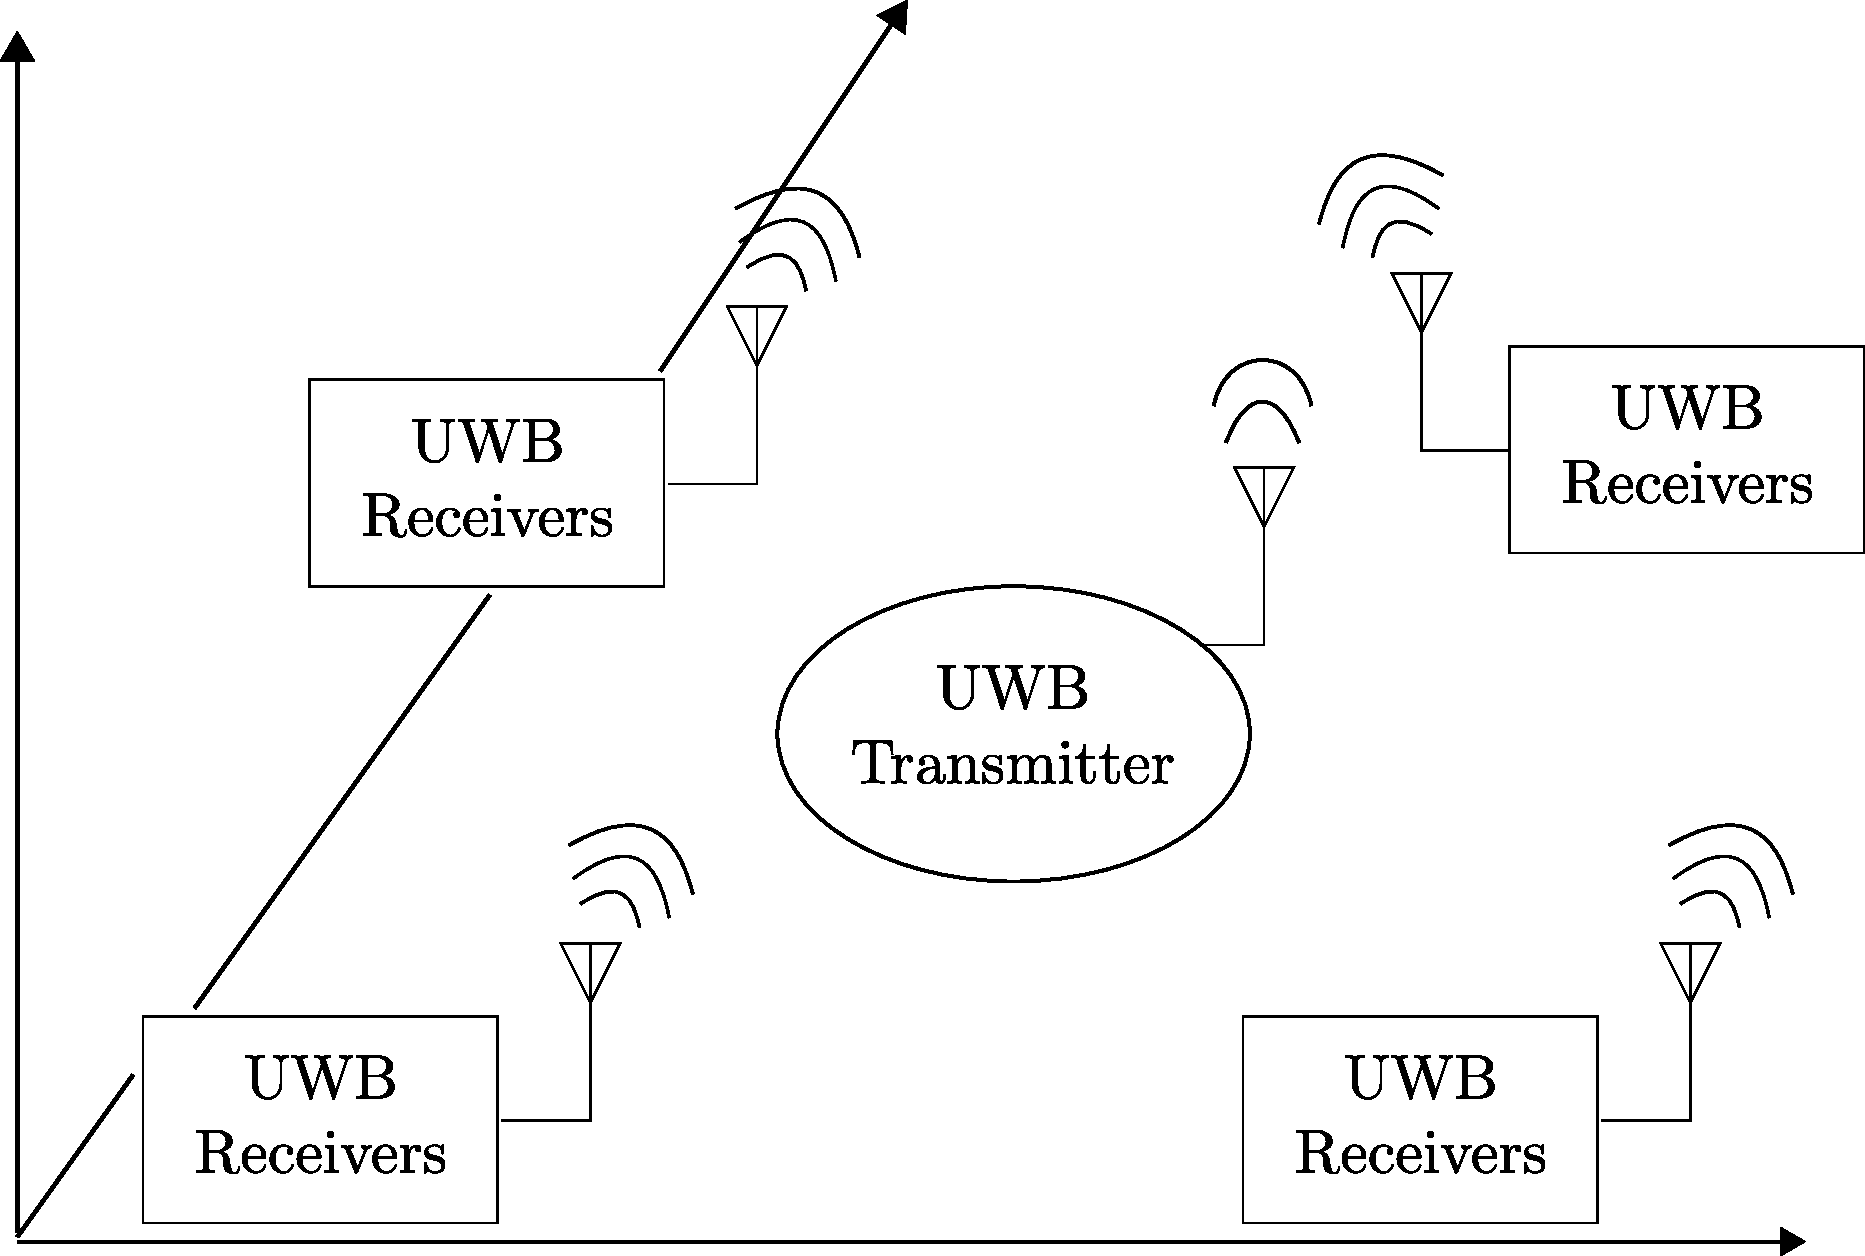
\includegraphics[width=2.7in]{pictures/uwb1.pdf}
\DeclareGraphicsExtensions.
\caption{Block diagram of typical UWB indoor communication system}
\label{uwb1}
\end{figure}

Ultra-wide band (UWB) communication is widely used in wireless communication and associated with features as extremely wide transmission bandwidth, low-power consumption, shared spectrum resources etc \cite{paredes2007ultra}. Among all applicable areas, one of the most popular application is impulse-radio ultra-wideband (IR-UWB) based communication in short range, where portable instruments such as wireless sensor networks (WSNs) can be used, involving indoor positioning, surveillance, and home automation etc. IR-UWB short range communication provides robustness to multipath fading environments even in low signal-to-noise (SNR) situations \cite{cassioli2002ultra}, and it meets the requirements of high data rate communication in battery supplied devices. 
However, high data rate transmission puts huge pressure on signal detection at ADCs at receivers, which indicates the sampling rate becomes a main bottleneck to the IR-UWB system. This part focuses on a popular application area in IR-UWB, that is the IR-UWB indoor positioning, aims at solving the bottleneck of sampling rate by using a recent novel technique termed compressed sensing (CS). Compressed sensing is a novel paradigm which applies randomly sampling and sparse reconstruction, which enables a possible reconstruction strategy for sparse signals from a relatively small group of random measurements. It indicates that CS based IR-UWB systems can possibly detect high frequency sparse signals under a sub-Nyquist sampling rates that far below the Nyquist rate (twice the IR-UWB bandwidth). This result is advantageous which releases the bottleneck of the large bandwidth constraints on ADC at UWB receivers, and consequently reduces storage limits and improves energy efficiency in IR-UWB positioning systems.


\subsubsection{CS Receivers for UWB Positioning}

Recently some researches manage to embed CS reconstruction algorithms, e.g. revised orthogonal matching pursuit, at UWB receivers. These algorithms successfully improve the SNR of the received signal before they are sent to the stages of time of arrival (TOA) based positioning algorithm. Consequently, this method increases the performance of entire positioning accuracy \cite{banitalebi2014compressive}. For hardware implementation of new CS based UWB receivers, most of them apply the hardware structure termed the random demodulator (RD) \cite{kirolos2006analog}, and consequencely this new CS-UWB receivers successfully reduce the sampling rate significantly compared to Nyquist rate \cite{yang2011compressive}.

\begin{figure}[!t]
\centering
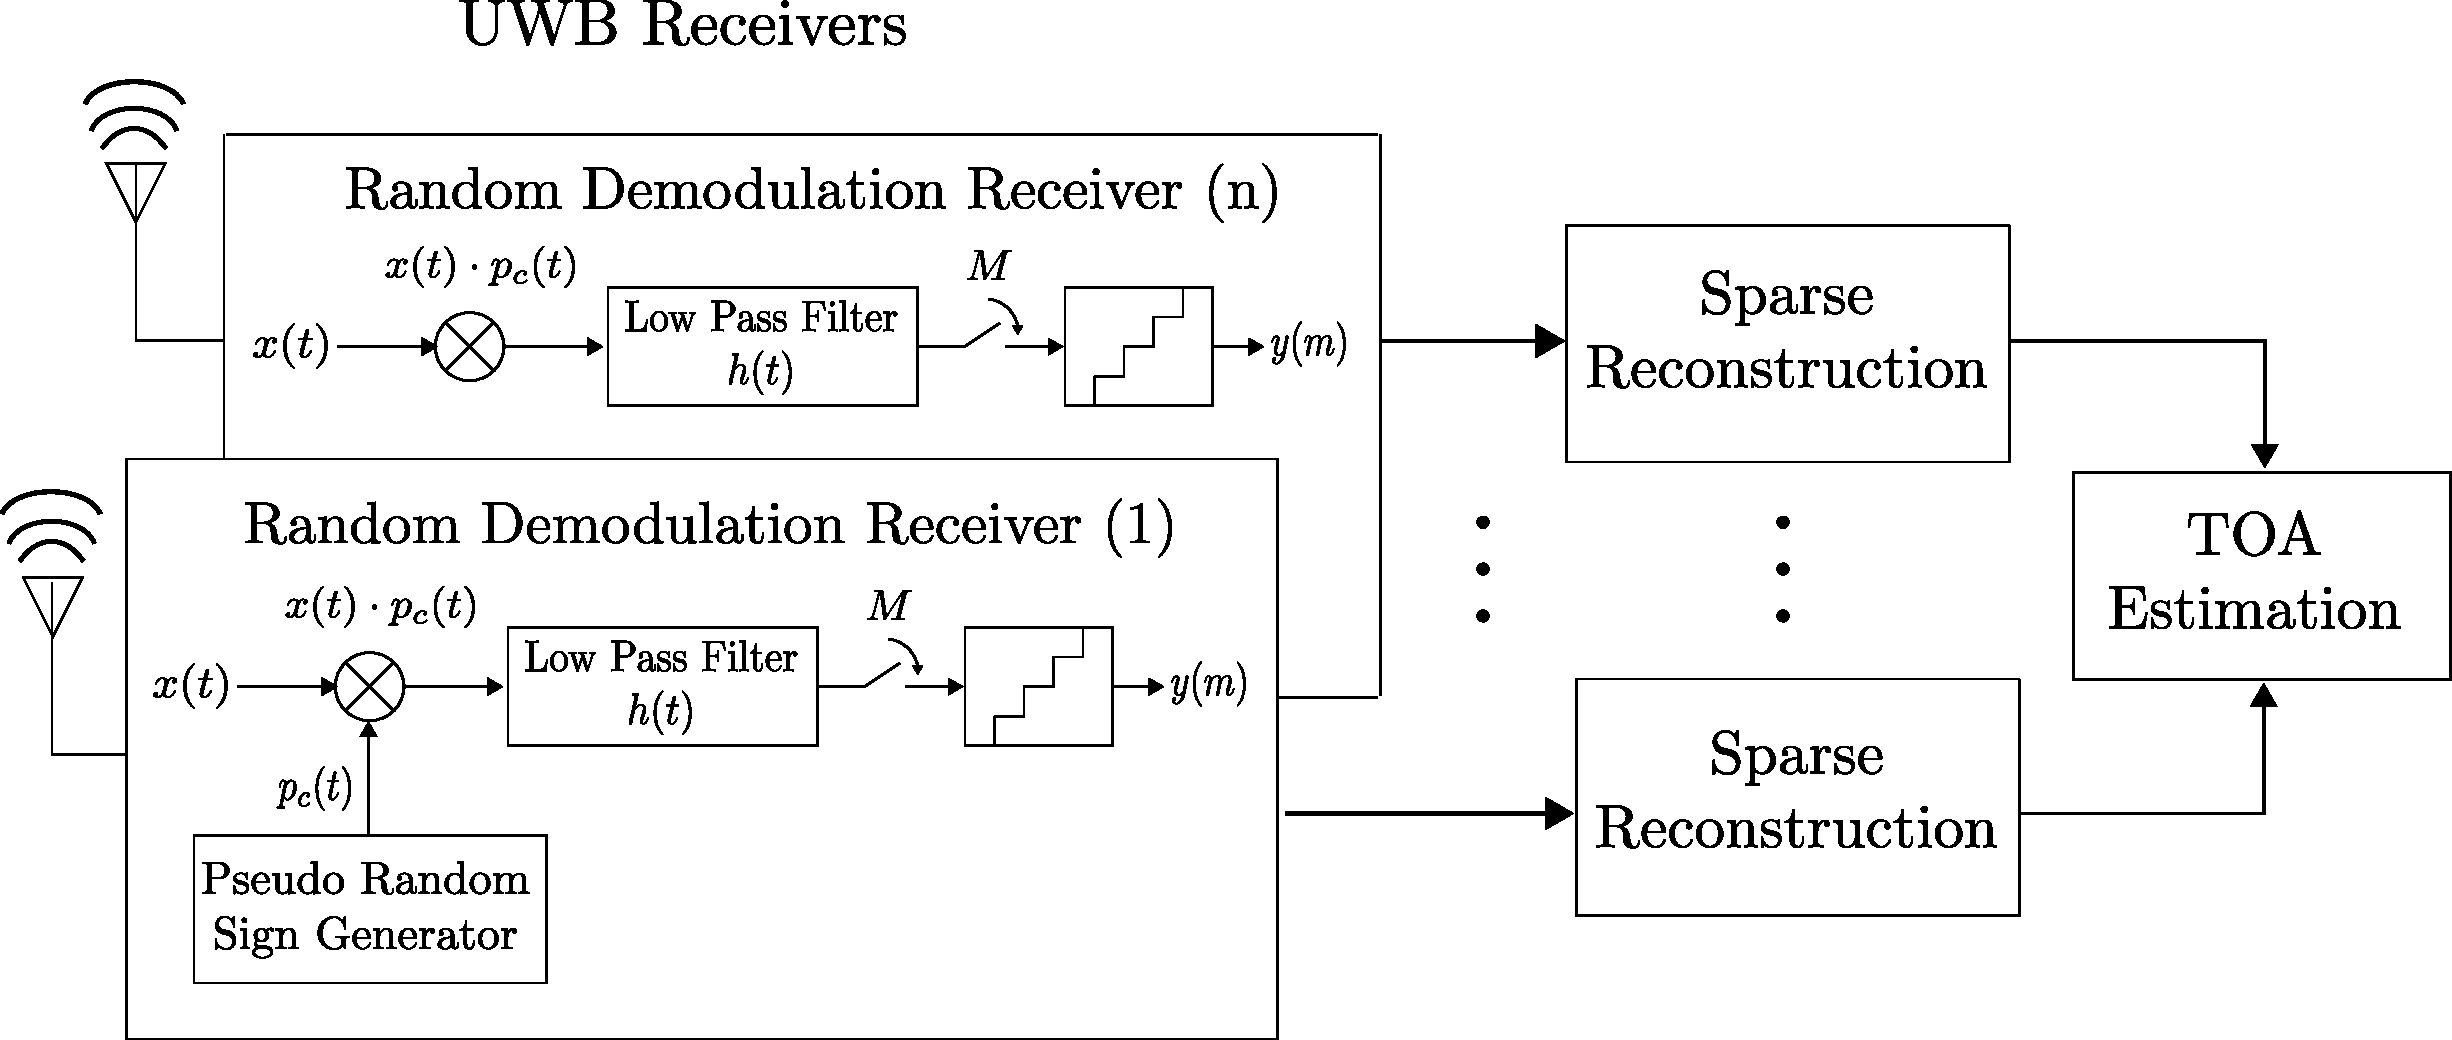
\includegraphics[width=3.5in]{pictures/cs-uwb-design1.pdf}
\DeclareGraphicsExtensions.
\caption{Block diagram of CS Receiver implemented by random demodulator (RD). The components of RD includes a pseudo-random sign generator (PRSG), a low-pass filter (LPF), and a sub-Nyquist ADC}
\label{cs-uwb-design1}
\end{figure}

In this system, each CS Receiver realizes the RD architecture that composed of a pseudo-random sign generator (PRSG), a low pass filter (LPF), and a sub-Nyquist rate analog-to-digital converter (ADC), shown in Fig.\ref{cs-uwb-design1}. Then the transmitted UWB signals are collected by group of low-rate distributed ADCs only using a minimal sampling rate of $1.7K(log(N/K))$ \cite{kirolos2006analog}, where $N$ stands for Nyquist rate and $K$ is the sparsity in transmitted UWB signals. Results in \cite{yang2013compressive} demonstrates that the new system successfully improves positioning accuracy. 

\subsubsection{CS Pre-Filtering for UWB Positioning}

On the other hand, some UWB positioning systems applies CS technique at the UWB transmitter and regarded it as a better solution than CS receivers on account of system hardware power efficiency. The new architecture contains CS pre-filtering at the transmitter, which is a psudo-random sequence based implementation of the CS random projection before UWB signals are transmitted \cite{zhang2009compressed}, shown in Fig.\ref{cs-uwb-design2}. Followed by distributed sub-Nyquist rate ADCs, the downsampled signals are collected for TOA based algorithm. Simulation result shows that the new CS transmitter for UWB positioning successfully reaches positioning performance of CS receivers. Besides it meanwhile saves more energy cost since it contains less hardware mixers than CS receiver based UWB system. In this model, the channel model is required for precise sparse reconstruction. Some researches embeds the framework of Bayesian into CS theory, and applied this technique to UWB channel estimation using a priori distribution.  

\begin{figure*}[!t]
\centering
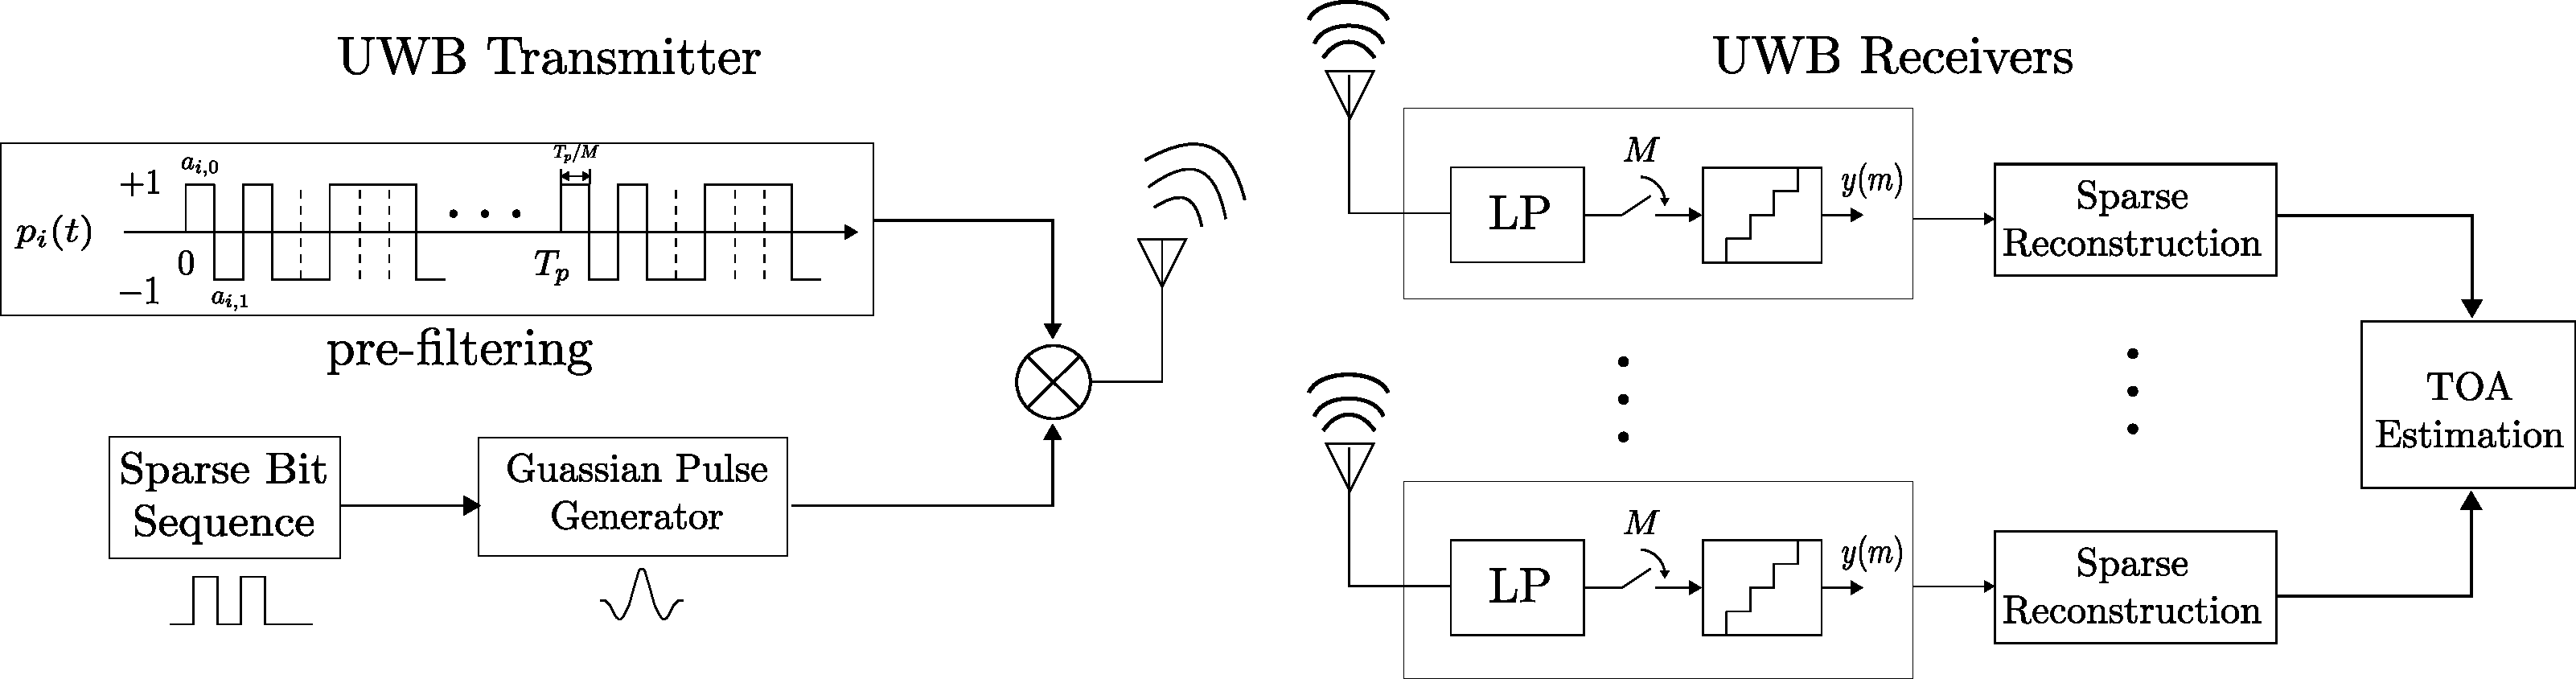
\includegraphics[width=6.0in]{pictures/cs-uwb-design2.pdf}
\DeclareGraphicsExtensions.
\caption{Block diagram of low-rate CS pre-filtering (LRCSPF) UWB positioning system.}
\label{cs-uwb-design2}
\end{figure*}
